%%%%%%%%%%%%%%%%%%%%%%%%%%%%%%%%%%%%%%%%%
% Beamer Presentation
% LaTeX Template
% Version 1.0 (10/11/12)
%
% This template has been downloaded from:
% http://www.LaTeXTemplates.com
%
% License:
% CC BY-NC-SA 3.0 (http://creativecommons.org/licenses/by-nc-sa/3.0/)
%
%%%%%%%%%%%%%%%%%%%%%%%%%%%%%%%%%%%%%%%%%

%----------------------------------------------------------------------------------------
%	PACKAGES AND THEMES
%----------------------------------------------------------------------------------------

\documentclass{beamer}

\mode<presentation> {

% The Beamer class comes with a number of default slide themes
% which change the colors and layouts of slides. Below this is a list
% of all the themes, uncomment each in turn to see what they look like.

%\usetheme{default}
%\usetheme{AnnArbor}
%\usetheme{Antibes}
%\usetheme{Bergen}
%\usetheme{Berkeley}
%\usetheme{Berlin}
%\usetheme{Boadilla}
%\usetheme{CambridgeUS}
%\usetheme{Copenhagen}
%\usetheme{Darmstadt}
%\usetheme{Dresden}
%\usetheme{Frankfurt}
%\usetheme{Goettingen}
%\usetheme{Hannover}
%\usetheme{Ilmenau}
%\usetheme{JuanLesPins}
%\usetheme{Luebeck}
\usetheme{Madrid}
%\usetheme{Malmoe}
%\usetheme{Marburg}
%\usetheme{Montpellier}
%\usetheme{PaloAlto}
%\usetheme{Pittsburgh}
%\usetheme{Rochester}
%\usetheme{Singapore}
%\usetheme{Szeged}
%\usetheme{Warsaw}

% As well as themes, the Beamer class has a number of color themes
% for any slide theme. Uncomment each of these in turn to see how it
% changes the colors of your current slide theme.

%\usecolortheme{albatross}
%\usecolortheme{beaver}
%\usecolortheme{beetle}
%\usecolortheme{crane}
%\usecolortheme{dolphin}
%\usecolortheme{dove}
%\usecolortheme{fly}
%\usecolortheme{lily}
%\usecolortheme{orchid}
%\usecolortheme{rose}
%\usecolortheme{seagull}
%\usecolortheme{seahorse}
%\usecolortheme{whale}
%\usecolortheme{wolverine}

%\setbeamertemplate{footline} % To remove the footer line in all slides uncomment this line
%\setbeamertemplate{footline}[page number] % To replace the footer line in all slides with a simple slide count uncomment this line

\setbeamertemplate{navigation symbols}{} % To remove the navigation symbols from the bottom of all slides uncomment this line
}

\usepackage{graphicx} % Allows including images
\usepackage{booktabs} % Allows the use of \toprule, \midrule and \bottomrule in tables

%----------------------------------------------------------------------------------------
%	TITLE PAGE
%----------------------------------------------------------------------------------------

\title[Github]{Découverte de git par la pratique} % The short title appears at the bottom of every slide, the full title is only on the title page

\author{Ugo Proietti} % Your name
\institute[UMONS] % Your institution as it will appear on the bottom of every slide, may be shorthand to save space
{
Université de Mons \\
CPUMons \\ % Your institution for the title page
\medskip
\textit{ugo.proietti@student.umons.ac.be} % Your email address
}
\date{23 février 2022} % Date, can be changed to a custom date

\begin{document}

\begin{frame}
\titlepage % Print the title page as the first slide
\end{frame}

\begin{frame}
\frametitle{} % Table of contents slide, comment this block out to remove it
\tableofcontents % Throughout your presentation, if you choose to use \section{} and \subsection{} commands, these will automatically be printed on this slide as an overview of your presentation
\end{frame}

%------------------------------------------------
%	PRESENTATION SLIDES
%------------------------------------------------

%------------------------------------------------
\section{Que sont git et GitHub} % Sections can be created in order to organize your presentation into discrete blocks, all sections and subsections are automatically printed in the table of contents as an overview of the talk
%------------------------------------------------

\begin{frame}\frametitle{Git $\neq$ GitHub}
Git est un outil permettant aux développeurs de gérer les différentes versions de leur programme et de collaborer sur le même projet.\\~\\

GitHub est un site permettant d'héberger des repository git. Il en existe d'autres tels que GitLab ou Bitbucket.
\end{frame}

%------------------------------------------------

\begin{frame}\frametitle{Git}
\begin{itemize}
    \item Gestion de versions
    \item Collaboration avec d'autres développeurs
    \item Gestion de conflits
    \item Développement non-linéaire
\end{itemize}
\end{frame}

%------------------------------------------------

\begin{frame}\frametitle{GitHub}
\begin{itemize}
    \item Un des sites les plus connus
    \item GitHub pro gratuit pour étudiant
    \item Actions pour automatiser ce qu'on veut
    \item Arctic code vault
\end{itemize}
\end{frame}

%------------------------------------------------
\section{Comment utiliser les outils} % Sections can be created in order to organize your presentation into discrete blocks, all sections and subsections are automatically printed in the table of contents as an overview of the talk
%------------------------------------------------

\begin{frame}\frametitle{Installer git et/ou GitHub Desktop}
    Pour la version CLI, il suffit d'avoir git installé sur sa machine (déjà installé sur Linux ; Git Bash pour windows). Il faudra ensuite générer une clé SSH et l'ajouter sur GitHub.com \\~\\
\end{frame}

%------------------------------------------------

\begin{frame}\frametitle{Créer un repository}
    À faire depuis le site GitHub.com. Le site donnera les instructions à réaliser avec git CLI. \\~\\
\end{frame}

%------------------------------------------------

\begin{frame}\frametitle{Éditer un repository}
    \begin{itemize}
    \item Depuis GitHub.com, allez sur le repository concerné et cliquez sur le bouton \textbf{Fork}. Pour la présentation, faites-le avec \textbf{cpumons/workshop-git}\\
        \item Clonez sur votre machine le nouveau repository \\
        \item Faites vos modifications (voir slide suivante) \\
        \item Créez une pull request en cliquant sur \textbf{Contribute}
        \item (Gérez les conflits, voir slide 10)
    \end{itemize}
\end{frame}

%------------------------------------------------

\begin{frame}\frametitle{Commandes de base}
    \begin{itemize}
        \item \$ vi 2023.md
        \item \$ git add 2023.md
        \item \$ git commit -m "Ma modification"
        \item \$ git push
    \end{itemize}

    Retournez à la dernière étape de la slide précédente
\end{frame}

%------------------------------------------------

\begin{frame}[fragile]\frametitle{Gestion des conflits}
    Si deux développeurs modifient le même fichier, un conflit va apparaître.
    \begin{verbatim}
    <<<<<<< HEAD
        Mon code
    =======
        Code précédent
    >>>>>>> Autre branche
    \end{verbatim}
\end{frame}

%------------------------------------------------

\begin{frame}\frametitle{Branches}
    \begin{center}
        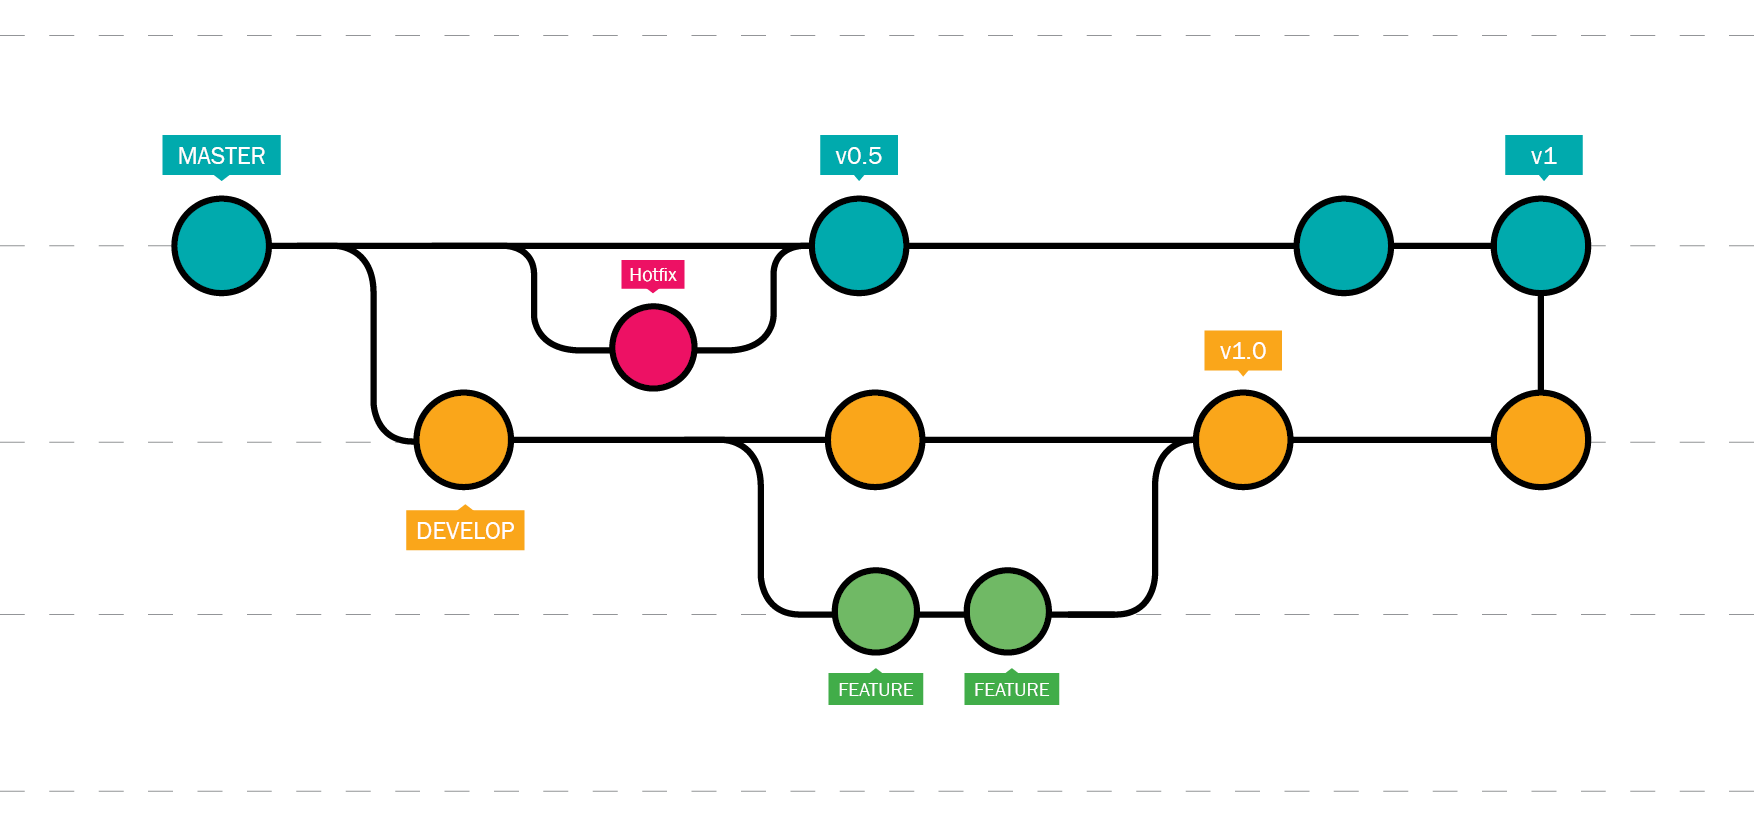
\includegraphics[scale=0.185]{branch.png}
    \end{center}
    \begin{itemize}
        \item \$ git branch
        \item \$ git checkout
    \end{itemize}
\end{frame}

%------------------------------------------------

\begin{frame}\frametitle{.gitignore}
    Fichier stockant une liste d'exceptions. \\~\\

    Des générateurs existent, par exemple gitignore.io
\end{frame}

%------------------------------------------------
\section{Cas pratiques} % Sections can be created in order to organize your presentation into discrete blocks, all sections and subsections are automatically printed in the table of contents as an overview of the talk
%------------------------------------------------

\begin{frame}\frametitle{Deux exemples à votre disposition}
    Il existe 2 repository sur le GitHub de CPUMons : \textbf{cpumons/gradle-template} et \textbf{cpumons/latex-template}. \\~\\

    Ces 2 ressources sont très utiles pour utiliser Gradle et Latex. Voir démo.
\end{frame}

%------------------------------------------------

\end{document}
